%Correct the file name.
%X: book number
%Y: part number
%ZZZ: page number in three digits. So page 3 would be 003.

\documentclass[11pt]{amsbook}

\usepackage{../HBSuerDemir}	% ------------------------
\usepackage{amsmath, wrapfig}

\begin{document}
\hPage{b2p2/413}
\begin{wrapfigure}{r}{.5cm}
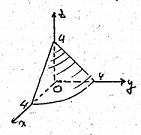
\includegraphics[width=0.45\textwidth]{images/b2p2-413-fig01}
\end{wrapfigure}


\underline{Solution}.

$\\I_1=\int \int_{S_{yz}}^{} x^2z dydz=\int_{0}^{4}\int_{0}^{4-y} x^2z dydz$

\[
	= \int_{0}^{4}\int_{0}^{4-y} \Big( (z-4)^2-y^2 \Big)z dzdy
\]

\[
	= \int_{0}^{4}\int_{0}^{4-y} ( (z^3-8z^2+16z-y^2z )dzdy
\]

\[
	= \int_{0}^{4} \frac{z^4}{4} -\frac{8}{3}z^3 + \frac{16-y^2}{z} z^2
	\bigg|_0^4
	dy\\
\]

\begin{wrapfigure}{r}{.5cm}
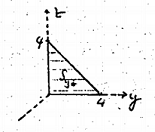
\includegraphics[width=0.45\textwidth]{images/b2p2-413-fig02}
\end{wrapfigure}

$\\A=\Big( (4-y)^2 \frac{(4-y)^2}{4} - \frac{8}{3} (4-y) + \frac{16-y^2}{2} \Big)$

\[
	= (y-4)^2 \frac{-3y^2+8y+16}{12}
\]

\[
	= - \frac{1}{2} (3y^4-32y^3+96y^2-256)
\] 

\begin{wrapfigure}{r}{.5cm}
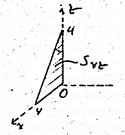
\includegraphics[width=0.45\textwidth]{images/b2p2-413-fig03}
\end{wrapfigure}

$I_1= -\frac{1}{12} \Big(\frac{3}{5} y^5-8y^4+32y^3-256y \Big)_0^4=\frac{512}{15} $

$ I_2=\int\int_{S_{xz}} y^2x dzdx=\int_0^4\int_0^(4-z) y^2xdxdz=I_1$ \\
$ I_3=\int\int_{S_{xy}} z^2y dxdy = \int_0^4\int_0^{\sqrt{16-x^2}} z^2y dydx $

\[
	=\int_0^4\int_0^{\sqrt{16-x^2}} (4+\sqrt{x^2+y^2}) dydx
\]



\[
	=4\int_0^4\int_0^{\sqrt{16-x^2}} dydx + \int_0^{\pi/2}\int_0^4 r.r drd\vartheta
\]

\[
	=16\pi + \frac{32}{3} \pi=\frac{80}{3} \pi
\]

$I=\frac{2.512}{15} +\frac{80}{3} \pi.$

\begin{wrapfigure}{r}{.5cm}
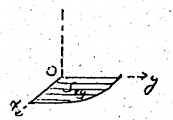
\includegraphics[width=0.45\textwidth]{images/b2p2-413-fig04}
\end{wrapfigure}


\end{document}  

%==== templates ====

%==== environments ====

%\begin{figure}[htb]
%	\centering
%	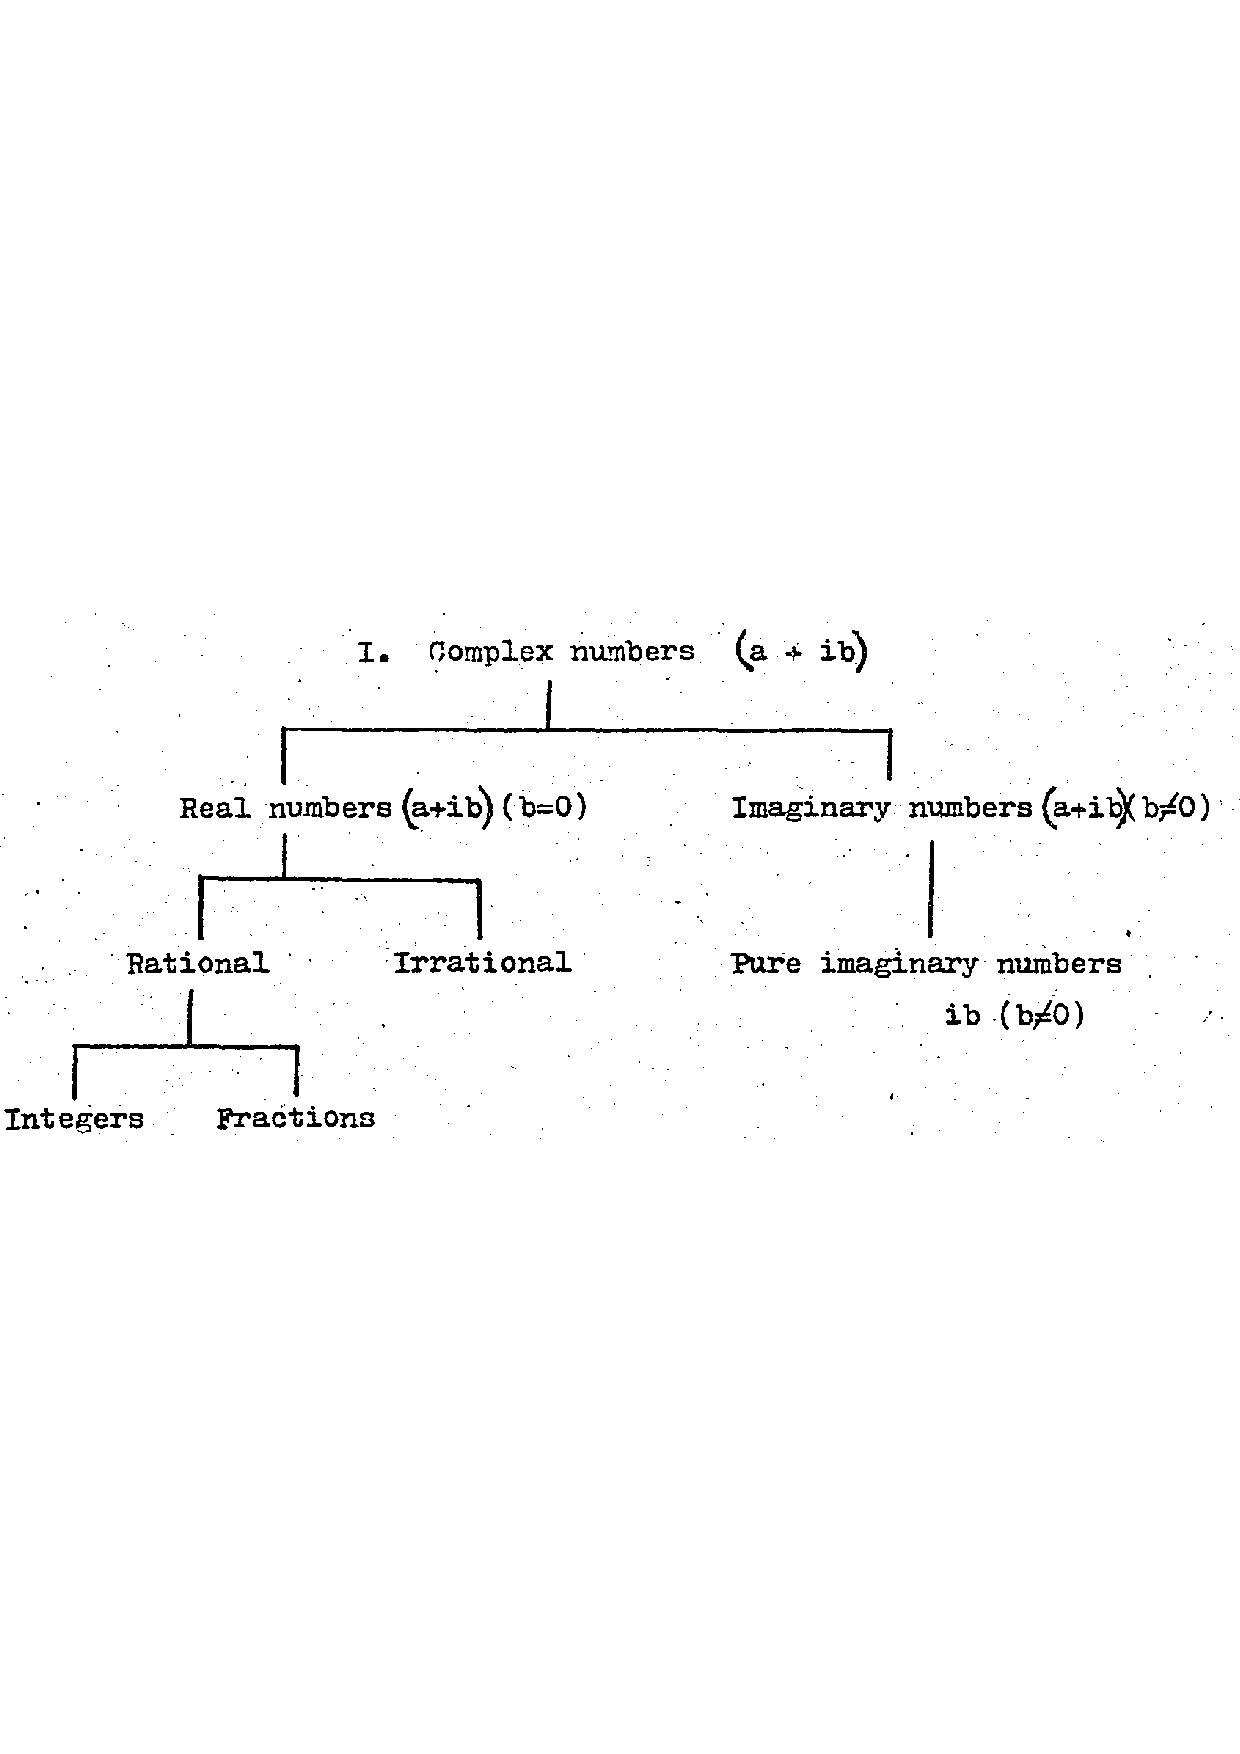
\includegraphics[width=0.9\textwidth]{images/SD-1-1p15A}
%	\caption{Classification of complex numbers}
%	\label{fig:classificationOfComplexNumbersA}
%\end{figure}

%\begin{center}
%\begin{tabular}{cc}
%\end{tabular}
%\end{center}

%\begin{exmp}
%\begin{hSolution}
%\end{hSolution}
%\end{exmp}

%\begin{hEnumerateAlpha}
%\end{hEnumerateAlpha}

%\begin{hEnumerateRoman}
%\end{hEnumerateRoman}

%$
%\begin{bmatrix}
%\end{bmatrix}
%$

%\frac{aaaa}{bbb}
%\frac{a_{n}}{b_{n}}
%\left( aaaa \right)
%\Longrightarrow

%\begin{multicols}{2}
%	bb
%\columnbreak
%	aa
%\end{multicols}
